\documentclass{procDDs}

\usepackage[utf8]{inputenc}                                                 % load packages only if necessary
%\usepackage[english, russian]{babel}
\usepackage[usenames]{color}


\title{Reconstruction of the Seabottom Reflection Coefficient}

\author{\textbf{Evgeny O. Kovalenko}}% List of authors with the
{Far Eastern Federal University, Vladivostok, Russia}                 % same affiliation,
% lecturer given in bold
{kovalenko.eo@dvfu.ru}                                   % 

\author{Igor V. Prokhorov, Andrey A. Sushchenko}% List of authors with the
{Institute for Applied Mathematics, FEB RAS, Vladivostok, Russia, \\ 
	Far Eastern Federal University, Vladivostok, Russia}                 % same affiliation,
% lecturer given in bold
{prokhorov@iam.dvo.ru, sushchenko.aa@dvfu.ru}                                   % e-mail of lecturer
%
%                                                 % it is important not to have
%                                                 % blank lines between the
%                                                 % \author and \coauthor
%

\begin {document}

\maketitle

\index{Kovalenko, E.O.}                              % write this for each author
\index{Prokhorov, I.V.}                              % to generate the index
\index{Sushchenko, A.A.}   
%
\def\k{\mathbf{k}}
\def\n{\mathbf{n}}
\def\x{\mathbf{x}}
\def\y{\mathbf{y}}
\def\r{\mathbf{r}}
\def\p{\mathbf{|}}
\def\z{\mathbf{z}}
\def\V{\mathbf{V}}
\def\Vt{\mathbf{V}t}
\def\exp{\text{exp}}

\begin{abstract}
	The kinetic model, describing sound propagation in the ocean with diffuse reflection by Lambert's cosine law on the bottom surface, is considered. Based on it the inverse problem of bottom scattering reconstruction is formulated.
	The inverse problem is reduced to solving the Fredholm integral equation of the first kind. An iterative algorithm solving it is developed. Numerical experiments reconstruction of the seabottom scattering coefficient at different width of directivity pattern are carried out.
\end{abstract}

\section{Introduction}
There is mainstream problem in the World Ocean research which relates to conservation and rational use of its resources. Nowadays, ocean can barely afford to many times increased the anthropogenic influence. Its variations is required a permanent monitoring. One of the most effective method of registration for local changes is survey of a seabottom and a water column using by autonomus unmanned vehicle which equipped by a side-scan sonar (SSS). The principle of sonar is based on emitting and detecting of the reflected echosignal. There are several approaches for the description of this process. The wave models, taking into account an amplitude and a phase of the propagated signal, is most common use. However, if wavelength is comparable to the sampling scale then the beam signal propagation theory is also valid \cite{Turner, Zurk}. It is based on the kinetic model of the transfer acoustic radiation in the randomly inhomogeneous media \cite{AF2015, SPIE_KOV}. The main advantage of this model is taking into account the middle scattering in the media which is constitute about 10\% of the total attenuation in a demersal layer, according to the practical research I.B. Andreeva \cite{Andreeva}. The influence of the volume scattering on the propagating signal is widely studied in the previous works. For instance, in paper \cite{AF2015} the problem of the determination the seabottom scattering coefficient based on the received signal by sonar is considered. That problem was solved using by following approximations. There are the single scattering in the media, narrow directivity pattern of the receiving antenna and a pointwise source. Authors deduced an explicit formula for the determination of the seabottom scattering coefficient which is taking into account the additive correction to the volume scattering in the total signal. Further evolution of this problem is continued in paper \cite{SPIE_KOV} in which authors used a source is been close to the real experiments. It emits parcels during finite time interval. Thus, authors reduced the reconstruction problem to the Fredholm integral equation of the first kind in the left side of which is a total measured signal by SSS,  on the other side is unknown function, describing inhomogeneous of the seabottom surface.

There are so many papers about solving the Fredholm integral equation of the first kind. The most ones were based on the researches by A.N. Tikhonov and A.B. Bakushinskii \cite{Tikhonov, Baku}. Further, authors considered papers which is the most suitable for the specifics of the problem studying. It is worth to note authors research the problem with a receiver equipped by  a wide directivity pattern. In \cite{PRUAC} authors solved one using by the narrow directivity pattern approximation which leads to the object defocusing of the seabottom reconstruction. However, the solution of the directivity diagram has a small aperture.

Highly successful convolution algorithms for the reconstruction of  the Earth surface  using by a high-resolution satellite images are developed in the works of Shcherbinina N. V. \cite{Shcherbinina}. Method is based on using the frequency for the improving image sharpness. This approach could be applicable for the time spectrum also.

In paper \cite{p2} the focusing problem of laser radiation is solved in the approximation of the geometric optic. Authors were obtained the condition that if the incident radiation have a central symmetry and small domain of irradiation then problem is solvable.

In paper \cite{p3} authors interpreted the blur and defocusing as additive space-invariant distortion. The problem is solved using by the Fourier transform decomposition combined with the regularization.

In this paper authors develop a generalized algorithm of object focusing for the reconstruction of seabed scattering coefficient based on the received echosignal by SSS equipped by the widely directivity pattern. Thus, a solution of the Fredholm integral equation of the first kind is reduced to the solving of SLE by an iterative method combined with the regularization.

\section{Formulation of the problem}
\begin{figure}[h!]\center
	
	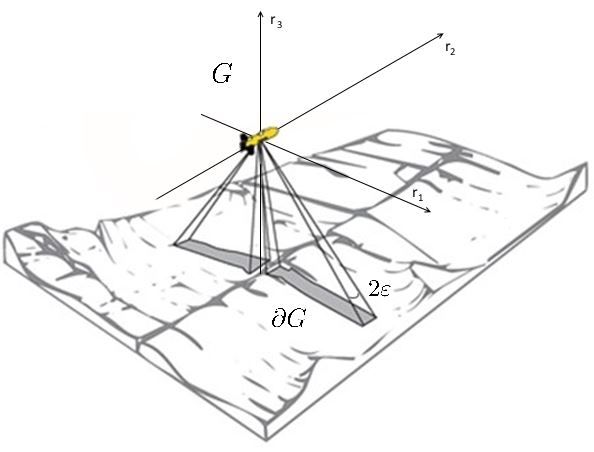
\includegraphics[width=1\linewidth]{gbo.jpg}
	\caption{Autonomous underwater vehicle with side-scan sonar on board}
	\label{ris:gbo}
\end{figure}
Propagation of acoustic waves on the tens order kHz frequencies in the fluctuating ocean is described by radiation
transfer equation \cite{AF2015, SPIE_KOV,SMJ2015, Prokh_Sush_Kim_2017}:
\begin{multline}
	\label{model}
	\frac{1}{c} \frac{\partial I}{\partial t} + \k \cdot \nabla I(\r,\k,t) + \mu I(\r,\k,t) = \\
	\frac{\sigma}{4 \pi} \int\limits_{\Omega} I(\r,\k',t) d\k' + J(\r,\k,t).
\end{multline}
Here $\r \in \mathbb{R}^3, t \in [0, T]$ and wave vector $\k$ belongs to the unit sphere $\Omega := \{\k \in \mathbb{R}^3: |\k| = 1\}$. The function $I(\r,\k, t)$ denotes the wave energy of flux density at time $t$  at the point $\r$ which propagates in the direction $\k$  with velocity $c$. $\mu$ and $\sigma$ denote the attenuation and the scattering coefficients, respectively, and the function $J$ describes the sources of wave field.

Sonar signal is propagated in the medium $G:=\{\r \in \mathbb{R}^3:r_3 > -l\}$, which is top half-space bounded by the surface $\partial G = \gamma := \{\y \in \mathbb{R}^3: y_3 = -l \}$, interpreted as the bottom of the ocean. And let $\textbf{n}(\y)$ --- outer normal to the boundary of the domain $G$. 

Further, authors consider the case of an isotropic pointwise source which moves with constant velocity $V$ along $r_2$ axis and emits a pulse parcels in times $t_i$, $\overline{1,m}$ with intensity $J_i$, respectively: 
\begin{equation}
\label{source}
J(\r,\k, t) = \delta(\r - \V t)\sum\limits_{i=0}^{N} J_i \delta(t-t_i).
\end{equation}
Here, $\delta$ denotes Dirac delta function, $\chi_{[a,b]}$ is characteristic function of interval $[a,b]$.

Assume, sources in medium are missing before initial time
\begin{equation}
\label{init_cond}
I\rvert_{t=0}=0.
\end{equation}

Let, $\Omega^\pm = \{\k \in \Omega: \pm k_3 < 0\}$ then the reflective properties of $\partial G$  are determined by diffuse reflection by the Lambert’s cosine law \cite{SPIE_KOV, Prokh_Sush_Kim_2017}:
\begin{equation}
\label{boundary_condition}
I(\y,\k) = \frac{\sigma_d}{\pi} \int\limits_{\Omega ^+}|\n(\y)\cdot \k'| I(\y,\k') d\k' ,
\end{equation}
where  $\y \in \partial G, \k \in \Omega^-$.


Let, $\Gamma = \{ (\Vt, \k, t): \k \in \Omega, t \in (0,T) \}$  then measuring of the receiving signal on $\Gamma$ is a sum of the signal, caused by the reflection from the bottom surface, and a signal scattered by the inhomogeneities of the medium $G$:
\begin{equation}
	\label{sum_sig}
	I^\pm(t) = \int_{\Omega} S^\pm(\k) I|_{\Gamma}(\Vt, \k, t)d\k.
\end{equation}
Here, $S^+(\k)$ and $S^-(\k)$ denote the directivity pattern of the receiving antenna on the starboard and portside, respectively. Further, authors consider the case of a narrow directivity pattern of the receiving antenna, focused on orthogonal plane to vehicle path:
\begin{equation}
\label{diagram}
S^\pm(\k) = \chi_{[0,\mp1]}(k_1)  \exp(-k_2^2/\sin^2(\varepsilon)),
\end{equation}
where, $\varepsilon $ - angle of the width of directivity pattern.

\section{Determination of the bottom scattering coefficient}


As already noted in the introduction in the previous works of the authors of \cite{AF2015, SPIE_KOV}, the effect of volume scattering on the quality of reconstructed images of the seabed was investigated. In this paper we will focus our attention on the problem of restoring the  function $\sigma_d$ for a broad radiation pattern and a finite pulse length.

The authors consider the case when the receiving antenna detects signals from one sensing interval only. The decision was presented as (\ref{model}) - (\ref{sum_sig}) as:
\begin{multline}
	\label{form}
	I^\pm_i(t) = \frac{1}{\pi}\int\limits_{-1}^{1}\sigma_d(y_1,y_2) S^{\pm}(\k) \times \\ \times
	\frac{ cl^2J_i \exp(-\mu c(t-t_i))dk_2}{|\Vt_i-\y|^2|\y-\Vt|y_1(t-t_i)|k_2 \V-c|},
\end{multline}
where, 
\begin{align*}
	|\Vt - \y| = \left|\dfrac{c(t-t_i)}{2}\left(1+\dfrac{V^2}{c^2}\right) \right|, \\
	|\x-\y| = \left|\dfrac{c(t-t_i)}{2}\left(1-\dfrac{V^2}{c^2}\right) \right|, \\
	y_1 = \sqrt{|\Vt-\y|^2 - l^2}.
\end{align*}
The equation (\ref{form}) describes receiving signal from SSS in the time $t$ from starboard and port side in the i-th sensing interval. Integral at the right side set on the seabottom domain from which the signal is reflected. Directivity pattern $S(\textbf{k})$ determines reflection area. $|Vt-y|$ denote the slant range for the receiver, whereas $|Vt_i-y|$   is the slant range for the source. $y_1$ is downrange.

\section{The Inverse Problem}
In practice there is interest of the solving an inverse problem for determination the seabottom scattering coefficient based on the received signal. Thus, the problem reduced to solving the Fredholm integral equation of the first kind (\ref{form}) on the function $\sigma_d$. It is well known that numerical solution of this equation is unsteady and depends on the kernel type, i.e. in (\ref{form}) is on the directivity pattern $S(\textbf{k})$. Further, authors consider two approaches to solving this equation.
\subsection{Narrow DP Approximation}
In previous paper\cite{SPIE_KOV} authors obtained the solution of equation (\ref{form}) in the approximation of narrow directivity pattern of the receiving antenna. In this case the solution of the equation reduces to the explicit formula for determination of the  seabottom reflection coefficient $\sigma_d$. Thus, for each time point $\y$ in the seabottom $\gamma$ there is only one receiving time $t$.
\begin{equation}
S^{\pm}(\k) = \chi_{0,\mp1}(k_1)\delta(k_2)
\end{equation}
Thus, the solution of (7) is
\begin{equation}
\label{sigma_form}
\sigma_d \left( y_1, y_2 \right) = \frac{2\pi}{J_icl^2} l_i^4 y_1 \exp(2\mu l_i)I^\pm(t).
\end{equation}
Here, a slant range $l_i=c(t-t_i)/2$, and $y_1=\sqrt{l_i^2-l^2}, y_2=Vt_i$.
The solution of (\ref{form}) in the form of (\ref{sigma_form}) is valid at small angles of the directivity pattern ($\varepsilon<0.1$). Unfortunatly, this assumption is not satisfied to the applicability of the formula (\ref{sigma_form}) and leads to the object defocusing on the bottom, i.e. the diameter of the objects increases several times, moreover, this effect is enhanced with increasing the sounding range.

\subsection{Discrete Method}
In the introduction authors outlined some methods for solving the problem.  The considered approaches are based on the iteration methods for solving an integral equation that imposes restrictions the kernel form. Convergence of the iterative process in equation (\ref{model}) is reached in a case $\varepsilon < 1.5^\circ$, that narrows the applicability classical methods. At that rate, authors generalize iterations with a regularization parameter.

From a mathematical point of view, the eq. (\ref{form}) is the Fredholm integral equation of the first kind on the function $\sigma_d$. Authors introduce the descrete method for solving it. That is to say authors define subdomains on the seabottom $\gamma$ in which $\sigma_d$ is constant. The discrete grid are defined  on the axes $y_1, y_2$.
\begin{align}
	\{ \big( y_1^p, y_2^q \big) \in\gamma: y_1^p = ph, y_2^q = qh \}, \notag \\ 
	p \in \overline{1, H}, q \in \overline{1, M}, 
\end{align}
where, $h$ is the grid spacing. In this way, the area limited of points $\big(y_1^p, y_2^q\big)$, $\big(y_1^{p+1}, y_2^q\big)$, $\big(y_1^p, y_2^{q+1}\big)$, $\big(y_1^{p+1}, y_2^{q+1}\big)$ $\sigma_d$  is constant and the equation (\ref{form}) reduces to:
\begin{equation}
\label{invI}
I(t_{ij}) = \sum \limits_{p=1}^{N} \sum \limits_{q=1}^{M} a_{ijpq}\sigma_d^{pq},
\end{equation}
where,
\begin{multline*}
	t_{ij} = t_i+j\tau, \tau = \frac{\Delta_t}{M}, a_{ijpq} = \\ 
	=  \int\limits_{-1}^{1}
	\frac{cl^2J_i \exp(-\mu c(t-t_i))dk_2}{|\Vt_i-\y|^2|\y-\Vt|y_1(t-t_i)|k_2 \V-c|}, \\
	\sigma_d^{pq} = \sigma_d(\textbf{y}^{pq}), \textbf{y}^{pq} = (y_1^p, y_2^q).
\end{multline*}
Eq. (\ref{invI}) is S-diagonal SLE. Parameter $s$ depends on the width of the receiver directivity pattern and on the source duration. For solving SLE (\ref{invI}) authors use  Seidel's method.
\section{Numerical experiments}
In the experiments, authors consider cases of the focusing on the different width of the directivity pattern. Authors use the formula (\ref{sigma_form}) as a zero iteration in Seidel's method, pictured on the figures (\ref{ris:desc1}) - (\ref{ris:desc6}) over character a). Experiments reach with the angle of the directivity pattern as  \{1, 2, 4, 8, 14, 40\} degrees. 
The probing parameters are represented in table \ref{table:name}.
\begin{table}[!ht]
	\begin{tabular}{|c|c|c|c|c|c|c|c|c|c|c|c|c|}
		\hline
		$\mu$,m$^{-1}$ & $\Delta t$,c & $c$,m/s & $J$ & $l$,m & $y_1$,m & $y_2$,m\\
		\hline
		0.018 & 0.4 & 1500 & 1 & 12 & [0,40] & [0, 40]\\ \hline
	\end{tabular}
	\label{table:name}
	\caption{Parameter values for the experiment}
\end{table}
The surface of the bottom is described by a function \ref{sigma_d} and is shown in the figure \ref{ris:dno}.
\begin{equation}
\scriptsize
\label{sigma_d}
\sigma_d(y_1, y_2) = 
\left\{
\begin{array}{ll}
0.3 , \quad  ((y_1-(12-b)a)-(y_2-6a))^2+\\ \quad \quad +\dfrac{3}{10}((y_2-(12-b)a)+(y_1-6a))^2<9a^2,  \\ \\
0.25, \quad \sqrt{(y_1-(8-b)a)^2+(y_2-9a)^2}<\dfrac{a^2}{4}, \\ \\
0.2 ,\quad  \sqrt{(y_1-(17-b)a)^2+(y_2-3a)^2}<\dfrac{a^2}{4}, \\ \\
0.1 , \quad \hbox{else.} \\
\end{array}%
\right.
\end{equation}
\begin{figure}[h!]\center
	
	
\includegraphics[width=0.3\linewidth]{dno.jpg}
	\caption{Exact solution}
	\label{ris:dno}
\end{figure}

Fig. \ref{ris:dno} shows the seabottom surface with a size of 20 m to 20 m. The sonar moves from the top left corner downwards, thereby setting the $ r_2 $ axis. Each line of the image corresponds to the new probing interval. From the physical point of view, the coefficient of the seabottom scattering is part of the reflected signal and is limited by the range [0;1]. Real experiments show that a part of the reflected signal does not exceed 35\%. At the fig. \ref{ris:dno} and further black color corresponds to 0, whereas white color to 0.35. Experiments with different width of the directivity pattern of the receiving antenna are presented below. The letters corresponds to the iteration number in the Seidel algorithm, starting from zero.

\begin{figure}[h!]\center%---------------ONE DEGREE---------------
	\begin{tabular}{cccc}
		
\includegraphics[width=0.2\linewidth]{k-img-5-1.jpg}&
		
\includegraphics[width=0.2\linewidth]{k-img-5-3.jpg}&
		
\includegraphics[width=0.2\linewidth]{k-img-5-4.jpg}&
		
\includegraphics[width=0.2\linewidth]{k-img-5-5.jpg}\\
		a & b & c & d \\
		
\includegraphics[width=0.2\linewidth]{k-img-5-6.jpg}&
		
\includegraphics[width=0.2\linewidth]{k-img-5-7.jpg}&
		
\includegraphics[width=0.2\linewidth]{k-img-5-8.jpg}&
		
\includegraphics[width=0.2\linewidth]{k-img-5-9.jpg}\\
		e & f & g & h		
	\end{tabular}
	\caption{Seabottom reconstruction with aperture of receiving antenna $\varepsilon=1^\circ$}
	\label{ris:desc1}
\end{figure}
\begin{figure}[h!]\center%---------------TWO DEGREE---------------
	\label{ris:desc2}
	\begin{tabular}{cccc}
		
\includegraphics[width=0.2\linewidth]{k-img-6-1.jpg}&
		
\includegraphics[width=0.2\linewidth]{k-img-6-3.jpg}&
		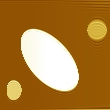
\includegraphics[width=0.2\linewidth]{k-img-6-4.jpg}&
		
\includegraphics[width=0.2\linewidth]{k-img-6-5.jpg}\\
		a & b & c & d \\
		
\includegraphics[width=0.2\linewidth]{k-img-6-6.jpg}&
		
\includegraphics[width=0.2\linewidth]{k-img-6-7.jpg}&
		
\includegraphics[width=0.2\linewidth]{k-img-6-8.jpg}&
		
\includegraphics[width=0.2\linewidth]{k-img-6-9.jpg}\\
		e & f & g & h \\
	\end{tabular}
	\caption{Seabottom reconstruction with aperture of receiving antenna $\varepsilon=2^\circ$ }
\end{figure}
\begin{figure}[h!]\center%---------------FOUR DEGREE---------------
	\begin{tabular}{cccc}
		
\includegraphics[width=0.2\linewidth]{k-img-7-1.jpg}&
		
\includegraphics[width=0.2\linewidth]{k-img-7-3.jpg}&
		
\includegraphics[width=0.2\linewidth]{k-img-7-4.jpg}&
		
\includegraphics[width=0.2\linewidth]{k-img-7-5.jpg}\\
		a & b & c & d\\
		
\includegraphics[width=0.2\linewidth]{k-img-7-6.jpg}&
		
\includegraphics[width=0.2\linewidth]{k-img-7-7.jpg}&
		
\includegraphics[width=0.2\linewidth]{k-img-7-8.jpg}&
		
\includegraphics[width=0.2\linewidth]{k-img-7-9.jpg}\\
		e & f & g & h
	\end{tabular}
	\caption{Seabottom reconstruction with aperture of receiving antenna $\varepsilon=4^\circ$}
	\label{ris:desc3}
\end{figure}
\begin{figure}[h!]\center%---------------EIGHT DEGREE---------------
	\begin{tabular}{cccc}
		
\includegraphics[width=0.2\linewidth]{k-img-9-1.jpg}&
		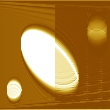
\includegraphics[width=0.2\linewidth]{k-img-9-3.jpg}&
		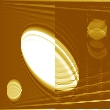
\includegraphics[width=0.2\linewidth]{k-img-9-4.jpg}&
		
\includegraphics[width=0.2\linewidth]{k-img-9-5.jpg}\\
		a & b & c & d\\
		
\includegraphics[width=0.2\linewidth]{k-img-9-6.jpg}&
		
\includegraphics[width=0.2\linewidth]{k-img-9-7.jpg}&
		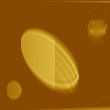
\includegraphics[width=0.2\linewidth]{k-img-9-8.jpg}&
		
\includegraphics[width=0.2\linewidth]{k-img-9-9.jpg}\\
		e & f & g & h
	\end{tabular}
	\caption{Seabottom reconstruction with aperture of receiving antenna $\varepsilon=8^\circ$}
	\label{ris:desc4}
\end{figure}
\begin{figure}[h!]\center%---------------FOURTEEN DEGREE---------------
	\begin{tabular}{cccc}
		
\includegraphics[width=0.2\linewidth]{k-img-13-1.jpg}&
		
\includegraphics[width=0.2\linewidth]{k-img-13-3.jpg}&
		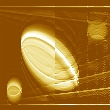
\includegraphics[width=0.2\linewidth]{k-img-13-4.jpg}&
		
\includegraphics[width=0.2\linewidth]{k-img-13-5.jpg}\\
		a & b & c & d\\
		
\includegraphics[width=0.2\linewidth]{k-img-13-6.jpg}&
		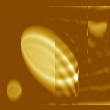
\includegraphics[width=0.2\linewidth]{k-img-13-7.jpg}&
		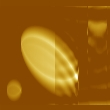
\includegraphics[width=0.2\linewidth]{k-img-13-8.jpg}&
		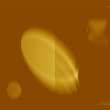
\includegraphics[width=0.2\linewidth]{k-img-13-9.jpg}\\
		e & f & g & h
	\end{tabular}
	\caption{Seabottom reconstruction with aperture of receiving antenna $\varepsilon=14^\circ$}
	\label{ris:desc5}
\end{figure}
\begin{figure}[h!]\center%---------------FOUTY DEGREE---------------
	\begin{tabular}{cccc}
		
\includegraphics[width=0.2\linewidth]{k-img-17-1.jpg}&
		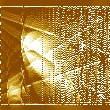
\includegraphics[width=0.2\linewidth]{k-img-17-3.jpg}&
		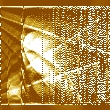
\includegraphics[width=0.2\linewidth]{k-img-17-4.jpg}&
		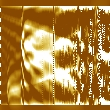
\includegraphics[width=0.2\linewidth]{k-img-17-6.jpg}\\
		a & b & c & d\\
		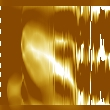
\includegraphics[width=0.2\linewidth]{k-img-17-8.jpg}&
		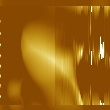
\includegraphics[width=0.2\linewidth]{k-img-17-10.jpg}&
		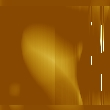
\includegraphics[width=0.2\linewidth]{k-img-17-11.jpg}&
		
\includegraphics[width=0.2\linewidth]{k-img-17-12.jpg}\\
		e & f & g & h
	\end{tabular}
	\caption{Seabottom reconstruction with aperture of receiving antenna $\varepsilon=40^\circ$}
	\label{ris:desc6}
\end{figure}
\begin{table}[h!]
	\begin{tabular}{|c|c|c||c|c|c|}
		\hline
		& $||\Delta\sigma||_2$ & $||\Delta\sigma||_\infty$ &
		& $||\Delta\sigma||_2$ & $||\Delta\sigma||_\infty$ \\ \hline
		a & 0.2666 & 0.0426 & e &  0.1730 & 0.0199\\ \hline
		b & 0.2051 & 0.0182 & f &  0.1832 & 0.0283\\ \hline
		c & 0.1781 & 0.0106 & g &  0.1890 & 0.0366\\ \hline
		d & 0.1778 & 0.0125 & h &  0.1952 & 0.0447\\ \hline
	\end{tabular}
	\label{table:desc1}
	\caption{Numerical error with $\varepsilon=1^\circ$}
\end{table}
\begin{table}[h!]
	\begin{tabular}{|c|c|c||c|c|c|}
		\hline
		& $||\Delta\sigma||_2$ & $||\Delta\sigma||_\infty$ &
		& $||\Delta\sigma||_2$ & $||\Delta\sigma||_\infty$ \\ \hline
		a & 0.3122 & 0.0749 & e &  0.1740 & 0.0207\\ \hline
		b & 0.2128 & 0.0337 & f &  0.1843 & 0.0319\\ \hline
		c & 0.1718 & 0.0191 & g &  0.1949 & 0.0432\\ \hline
		d & 0.1647 & 0.0134 & h &  0.2 & 0.0540\\ \hline
	\end{tabular}
	\label{table:desc2}
	\caption{Numerical error with $\varepsilon=2^\circ$}	
\end{table}
\begin{table}[h!]
	\begin{tabular}{|c|c|c||c|c|c|}
		\hline
		& $||\Delta\sigma||_2$ & $||\Delta\sigma||_\infty$ &
		& $||\Delta\sigma||_2$ & $||\Delta\sigma||_\infty$ \\ \hline
		a & 0.3333 & 0.1035 & e &  0.1653 & 0.0198\\ \hline
		b & 0.236 & 0.0627 & f &  0.1636 & 0.0266\\ \hline
		c & 0.2 & 0.0247 & g &  0.1819 & 0.0406\\ \hline
		d & 0.1634 & 0.0234 & h &  0.1983 & 0.0526\\ \hline
	\end{tabular}
	\label{table:desc3}
	\caption{Numerical error with $\varepsilon=4^\circ$}	
\end{table}
\begin{table}[h!]
	\begin{tabular}{|c|c|c||c|c|c|}
		\hline
		& $||\Delta\sigma||_2$ & $||\Delta\sigma||_\infty$ &
		& $||\Delta\sigma||_2$ & $||\Delta\sigma||_\infty$ \\ \hline
		a & 0.1959 & 0.0521 & e &  0.2 & 0.0299\\ \hline
		b & 0.2766 & 0.0424 & f &  0.1933 & 0.0324\\ \hline
		c & 0.2239 & 0.0319 & g &  0.1755 & 0.0399\\ \hline
		d & 0.1984 & 0.0291 & h &  0.1817 & 0.0477\\ \hline
	\end{tabular}
	\label{table:desc4}
	\caption{Numerical error with $\varepsilon=8^\circ$}
\end{table}
\begin{table}[h!]
	\begin{tabular}{|c|c|c||c|c|c|}
		\hline
		& $||\Delta\sigma||_2$ & $||\Delta\sigma||_\infty$ &
		& $||\Delta\sigma||_2$ & $||\Delta\sigma||_\infty$ \\ \hline
		a & 0.1926 & 0.0536 & e &  0.2225 & 0.0382\\ \hline
		b & 0.3106 & 0.0524 & f &  0.2 & 0.0355\\ \hline
		c & 0.3066 & 0.0428 & g &  0.2 & 0.0369\\ \hline
		d & 0.2505 & 0.0440 & h &  0.2 & 0.0423\\ \hline
	\end{tabular}
	\label{table:desc5}
	\caption{Numerical error with $\varepsilon=14^\circ$}
\end{table}
\begin{table}[h!]
	\begin{tabular}{|c|c|c||c|c|c|}
		\hline
		& $||\Delta\sigma||_2$ & $||\Delta\sigma||_\infty$ &
		& $||\Delta\sigma||_2$ & $||\Delta\sigma||_\infty$ \\ \hline
		a & 0.0886 & 0.4 & e &  0.1332 & 0.4\\ \hline
		b & 0.1438 & 0.4 & f &  0.1263 & 0.4\\ \hline
		c & 0.1444 & 0.4 & g &  0.1204 & 0.4\\ \hline
		d & 0.1384 & 0.4 & h &  0.1165 & 0.4\\ \hline
	\end{tabular}
	\label{table:desc6}
	\caption{Numerical error with $\varepsilon=40^\circ$}
\end{table}


%\section*{Conclusion}
As we can see, increasing the angle solution of the directivity pattern leads to increasing object diameter on the reconstruction image. For example, in the last experiments when $\varepsilon=40^\circ$ the diameter in the zeroth iteration increase in two times. It is worth to note that the method is applicable at small solutions of the directivity pattern, as can be seen from Fig. \ref{ris:desc2}. Further, in figures \ref{ris:desc3} - \ref{ris:desc5}, objects are compressed to their geometric center. However, the rough sampling leads to the appearance of artifacts that repeat the boundaries of the object. Moreover, each new iteration this effect is multiplied. To vanish boundary deformations, authors use a priori information on the admissible values of the seabottom scattering coefficient which allows to project the solution to allowable boundaries in each iteration. As you can see from the figures, the method qualitatively restores the boundaries of objects less than 8 iterations. With small solutions of directivity pattern, it is possible to obtain quantitative similarity. It is worth to note that in the limiting case at $\varepsilon = 40^\circ$ (Fig.-\ref{ris:desc6}) only the object with larger diameter is reconstructed due to the trace of the directivity pattern on the seabottom is larger than the diameter of small objects. Tables 2 --- 7 show the RMS and maximum errors in reconstructing the seabottom scattering coefficient at each iteration of the Seidel method. As can be seen from the experiments, the RMS error decreases to the certain threshold value, but after is increased. Thereby, the instability of the iterative method is confirmed. However, the visual representation of the image with further iterations only improves due to a discrepancy in absolute values with an exact solution. If in each iteration the solution is normalized to the maximum the method is absolutely applicable to any solutions of the directivity pattern.

\section*{Acknowledgements}
The research was supported by the Russian Science Foundation (Project No. 14-11-00079).

%  citations should be arranged by order of appearance

\begin {thebibliography}{9}

\bibitem{Turner} Turner, J.\,A., Weaver, R.\,L., 1994, 
Radiative transfer of ultrasound, 
\emph{The Journal of the Acoustical Society of America},  
Vol.\; {\bf 96}, No. {\bf 6}, pp.\; 3654--3674.

\bibitem{Zurk} Quijano, J.\,E., Zurk, L.\,M., 2009, 
Radiative transfer theory applied to ocean bottom modeling, 
\emph{The Journal of the Acoustical Society of America},  
Vol.\; {\bf 126}, No. {\bf 4}, pp.\; 711-723.

\bibitem{AF2015}  Prokhorov, I.\,V., Sushchenko, A.\,A., 2015, 
Studying the problem of acoustic sounding of the seabed using methods of radiative transfer theory, 
\emph{Acoustical Physics},
Vol.\; {\bf 61}, No. {\bf 3}, pp.\; 368--375.

\bibitem{SPIE_KOV} Kovalenko, E.\,O., Prokhorov, I.\,V., Sushchenko, A.\,A., 2016,
Processing of the information from side-scan sonar
\emph{Proceedings of SPIE - The International Society for Optical Engineering},
Vol.\;{\bf 10035}, Art. No. \;100352C

\bibitem{Andreeva} Andreeva,  I.\,B., 1995,
Comparative estimates of surface, bottom, and volume sound scattering in the ocean,
\emph{Akusticheskij Zhurnal},
Vol.\; {\bf 41}, No. {\bf 6} pp.\; 699--705.

\bibitem {Tikhonov} Tikhonov, A.\,N., 1943, 
Ob ustoichivosti obratnyh zadach [On the stability of inverse problems], 
\emph{Doklady Akademii Nauk USSR}, 
Vol. \;{\bf 39}, No. {\bf 5}, pp.\; 195--98 (in Russian).

\bibitem{Baku} Bakushinskii, A.\,B., Goncharskii, A.\,V., Levitan, S.\,Yu., 1988,
Fast linear iterative algorithms of image restoration,
\emph{USSR Computational Mathematics and Mathematical Physics},
Vol.\; {\bf 28}, No. { \bf 3},  pp.\; 210--213.

\bibitem {PRUAC} Prokhorov, I.\,V., Sushchenko A.\,A., 2015,
Analysis of the impact of volume scattering and radiation pattern on the side-scan sonar images, 
\emph{Proceedings of Meetings on Acoustics},
Vol.\; {\bf 24}, Art. No.\; 005007.

\bibitem {Shcherbinina} Ivashchuk, O.\,A., Shcherbinina, N.\,V., 2014,
Sravnitel'nyj analiz metodov vosstanovleniya pri korrekcii rezkosti na snimkah vysokogo razresheniya, 
\emph{Nauchnye vedomosti BelGU. Seriya: Istoriya. Politologiya. Ekonomika. Informatika.},
Vol.\; {\bf 21}, pp.\; 118--123.

\bibitem{p2}  Goncharskii, A.\,V., Stepanov, V.\,V., 1986,
Inverse problems of coherent optics, focussing in a line
\emph{USSR Computational Mathematics and Mathematical Physics},
Vol.\;{\bf 26}, No. {\bf 1},  pp.\; 50--57.

\bibitem{p3} Yagola, A.\,G., Koshev, N.\,A., 2008,
Restoration of smeared and defocused color images, 
\emph{Numerical Methods and Programming},
Vol.\;{\bf 9}, pp.\; 20--212 (in Russian).

\bibitem{SMJ2015} Prokhorov, I.\,V., Sushchenko,  A.\,A., 2015, 
On the well-posedness of the Cauchy problem for the equation of radiative transfer with Fresnel matching conditions,
\emph{Siberian Mathematical Journal},
Vol.\; {\bf 56}, No. {\bf 4}, pp.\; 736--745.

\bibitem{Prokh_Sush_Kim_2017} Prokhorov, I.\,V., Sushchenko,A.\,A., Kim, A., 2017, Initial Boundary Value Problem for the
Radiative Transfer Equation with Diffusion Matching Conditions
\emph{ Journal of Applied and Industrial Mathematics},  Vol. {\bf
	11}, Issue {\bf 1}, pp. 115--124.

\end{thebibliography}

\end {document}